

\chapter{Teoria della complessità ~\cite{3}~\cite{4}}
\label{complessita}
\section{Alfabeti e linguaggi}
\begin{definition}
    Un simbolo è un'entità primitiva astratta, lettere e caratteri sono simboli.
\end{definition}
\begin{definition}
    Un alfabeto $\Sigma$ è un insieme finito di simboli.
\end{definition}
\begin{definition}
    Una stringa è una sequenza finita di simboli, generalmente indicata con $w$, la sua lunghezza è indicata invece con $|w|$, la stringa vuota viene indicata con $\epsilon$ ed è tale che $|\epsilon|=0$.
\end{definition}
\begin{definition}
    Un linguaggio formale è un insieme di stringhe di simboli da un alfabeto $\Sigma$. \hfill \break
    L'insieme $\emptyset$ e l'insieme $\{\epsilon\}$ sono due linguaggi formali di qualunque alfabeto. \hfill \break
    Con $\Sigma^*$ si intende un linguaggio costituito da tutte le stringhe su un fissato alfabeto $\Sigma$. 
    Ad esempio se $\Sigma=\{0\}$ allora $\Sigma^*=\{\epsilon, 0,00,000,...\}$.
\end{definition}

\section{Definizione di macchina di Turing deterministica}
Una macchina di Turing M può essere definita come una quadrupla di elementi:
$$
M = (Q, \Sigma,q_0,\delta)
$$
dove:
\begin{itemize}
    \item $Q$: insieme finito di stati;
    \item $\Sigma$: insieme finito di simboli, contiene almeno i simboli $s_0=\$$ (blank) e il simbolo $s_1 = 0$ (tally);
    \item $\delta$: funzione di transizione, dati uno stato $q$ e un simbolo di nastro $X$, $\delta(q,X)$ restituisce una tripla $(p,Y,D)$:
    \begin{itemize}
        \item $p$: è lo stato successivo; 
        \item $Y$: è il simbolo di $\Sigma$ scritto nella cella visitata; 
        \item $D$: è una direzione, può essere $L$ o $R$; 
    \end{itemize}
    \item $q_0$: lo stato iniziale;
\end{itemize}

$\delta$ può essere definito come:
$$
\delta : Q \times \Sigma \rightarrow Q \times \Sigma \times \{L,R\}
$$

Definiamo a questo punto una descrizione istantanea (ID) come una quadrupla:
$$
\langle q,v,s,w\rangle
$$
dove: 
\begin{itemize}
    \item $q \in Q$: è lo stato in cui si trova la macchina; 
    \item $v,w \in \Sigma^*$: sono i caratteri diversi da blank a sinistra e destra della testina; 
    \item $s \in \Sigma$: è il simbolo letto dalla testina;
\end{itemize}
ad esempio:
$$
X_1 X_2 ... X_{i-1} q X_i X_{i+1}...X_n
$$
in cui: 
\begin{itemize}
    \item $q$ è lo stato della macchina di Turing; 
    \item la testina visita l'i-esimo simbolo da sinistra; 
    \item $X_1X_2...X_n$ è la porzione del nastro tra il simbolo diverso dal blank più a sinistra e quello più a destra;
\end{itemize}

Otteniamo quindi che le mosse di una macchina di Turing M sono definite mediante il simbolo $\vdash_M$.

\emph{}

Supponiamo che $\delta(q,X_i)=(p,Y,L)$ cioè la prossima mossa è verso sinistra, otteniamo: 
$$
X_1X_2...X_{i-1}qX_iX_{i+1}...X_n \vdash_M X_1X_2...X_{i-2}pX_{i-1}YX_{i+1}...X_n
$$

bisogna però tenere conto di due accorgimenti: 
\begin{itemize}
    \item se $i=1$ allora la mossa a sinistra fa muovere M verso il blank, ottenendo: 
    $$
    qX_1X_2...X_n \vdash_M pBYX_2...X_n
    $$
    \item se $i=n$ e $Y=\$$ allora il simbolo $\$$ scritto su $X_n$ si unisce alla sequenza di blank e non compare nella ID: 
    $$
    X_1X_2...X_{n-1}qX_n \vdash_M X_1X_2...X_{n-2}pX_{n-1}
    $$
\end{itemize}

Ci comportiamo allo stesso modo se la testina si muove a destra. Anche in questo caso si presentano le due eccezioni precedentemente descritte cambia solo il verso nel quale si vanno a scrivere i simboli. 

Per funzionare, la stringa di input viene posta sul nastro e la testina parte dal simbolo di input più a sinistra.
Se la macchina di Turing entra in uno stato accettante allora l'input è accettato, altrimenti no.
Si ha quindi che se $M=(Q,\Sigma,q_0, \delta)$ è una macchina di Turing, allora $L(M)$ è l'insieme di stringhe $w \in \Sigma^*$ tale che $q_0w\vdash^*\alpha p\beta$ per uno stato $p$ finale e qualunque stringa di nastro $\alpha$ e $\beta$.

\section{Arresto di una macchina di Turing}
Una macchina di Turing MdT si arresta se entra in uno stato $q$ visitando un simbolo $X$ e non ci sono mosse possibili in questa situazioni.
In tal caso otteniamo che $\delta(q,X)$ è indefinito.
Possiamo sempre presumere che MdT si arresti se accetta, tuttavia, non possiamo sempre richiedere che MdT si arresti. 
I linguaggi per i quali esiste una macchina di Turing che prima o poi si arresta (indipendentemente dal fatto che accetti o no), sono detti ricorsivi. 

Invece i linguaggi che possiamo accettare usando una macchina di Turing, ma che se non accettati non ci garantiscono che la macchina si fermi, sono denominati linguaggi ricorsivamente enumerabili. 

\section{Funzioni calcolabili da MdT}
Ad ogni MdT può essere associata una funzione calcolata dalla MdT.

\begin{definition}
Assumiamo di trattare solo funzioni sui naturali e di codificare i numeri naturali in una codifica unaria in cui ogni simbolo $n\in\mathbb{N}$ è rappresentato da $n+1$ $0$ consecutivi. 
Una funzione $f:\mathbb{N}^n\rightarrow \mathbb{N}$ è Turing-calcolabile se esiste una MdT M tale che partendo dalla configurazione iniziale: 
$$
...q_0\$x_1\$...\$x_n\$...
$$
se $f(x_1,...,x_n)$ è definita allora M termina nella configurazione:
$$
...\$\$\$...q_f\$f(x_1,...,x_n)\$...
$$
altrimenti M non termina, dove per ogni $(x_1,...,x_n)\in\mathbb{N}^n$, $x_1,...,x_n$, $f(x_1,...,x_n)$ sono le rappresentazioni in unario di $x_1,...,x_n$ e $f(x_1,...,x_n)$ mentre $q_f \in Q$ è tale che per cui $\delta(q_f, \$)$ è indefinito. 
\end{definition}

\begin{definition}
Una funzione totale è una funzione definita per ogni input.
\end{definition}

\section{Macchine di Turing multinastro}
Una MdT multinastro è formata da un controllo finito e un numero $k$ finito di nastri. 
Ogni nastro è diviso in celle e ogni cella può contenere un simbolo dell'alfabeto.
L'insieme di simboli di nastro comprende un blank e ha un sottoinsieme definito di simboli di input. 
L'insieme degli stati ne comprende uno iniziale e un sottoinsieme di stati finali (accettanti). 
Una MdT multinastro inizia rispettando:
\begin{itemize}
    \item l'input si trova sul primo nastro; 
    \item tutte le altre celle contengono un blank; 
    \item il controllo si trova nello stato iniziale; 
    \item la testina del primo nastro è all'estremità sinistra dell'input; 
    \item le altre testine si trovano in celle arbitrarie siccome sono tutte blank; 
\end{itemize}

Una mossa su una MdT multinastro dipende dallo stato e dai simboli letti da ciascuna testina. 
In una mossa la macchina compie: 
\begin{itemize}
    \item il controllo entra in un nuovo stato; 
    \item su ogni cella visitata da una testina viene scritto un nuovo simbolo di nastro; 
    \item ogni testina si muove a sinistra o a destra oppure sta ferma, i movimenti sono indipendenti.
\end{itemize}

In questo caso la funzione di transazione cambia, ed è definita come: 
$$
\delta : Q \times \Sigma^k \rightarrow Q \times \Sigma^k \times \{L,R\}^k
$$
cioè è un estensione della definizione di $\delta$ per le MdT singolo nastro dove partendo da uno stato $q \in Q$ si guardano $k$ simboli (uno su ogni nastro) e restituisce una tripla formata da uno stato, $k$ simboli scritti nelle $k$ celle visitate e $k$ direzioni in cui si muovono i $k$ nastri.

\begin{theorem}
    Ogni linguaggio accettato da una MdT multinastro è ricorsivamente enumerabile.
\end{theorem}
\begin{proof}
    Sia $L$ un linguaggio accettato da una MdT con $k$ nastri, M. Simuliamo M con una MdT mononastro N il cui nastro è diviso in $2k$ tracce. 
    Metà delle tracce ($k$) replicano i nastri di M, ognuna delle restanti indica la posizione corrente della testina del corrispondente nastro di M.
\end{proof}

\section{Definizione di macchina di Turing nondeterministica}
Una macchina di Turing nondeterministica si distingue da quella deterministica in quanto la funzione $\delta$ associa a ogni stato $q$ un insieme di triple, definito come: 
$$
\delta(q,X) = \{(q_1, Y_1, D_1), (q_2, Y_2, D_2),...,(q_k,Y_k, D_k)\}
$$con $k$ intero finito. 

A ogni passo la N-MdT sceglie una delle triple come mossa.
Si ottiene che M accetta una stringa $w$ se c'è una sequenza di scelte che conduce dalla ID iniziale con $w$a una ID con stato accettante. 

\begin{theorem}
    Se $M_N$ è una macchina di Turing nondeterministica, esiste una macchina di Turing deterministica $M_D$ tale che $L(M_N)=L(M_D)$.
\end{theorem}

\section{$k-$MdT ~\cite{4}}
Una $k-$Mdt è una macchina di Turing con $k-$nastri.
Come ogni MdT è definita come $M=(Q, \Sigma, q_0, P)$ dove: 
\begin{itemize}
    \item $Q$: è l'insieme finito di stati e $q_0 \in Q$ è lo stato iniziale; 
    \item $\Sigma$: è l'alfabeto in cui assumiamo siano presenti almeno i simboli $\$$ (blank) e $\triangleright$ (first);
    \item L'insieme delle istruzioni $P$ che rappresenta una funzione di transazione $\delta$ che assumiamo essere una funzione totale: 
    $$
    \delta : Q \times \Sigma^k \rightarrow (Q \cup\{h,yes,no\})\times (\Sigma \times \{L,R,F\})^k
    $$
    \item $h,yes,no$ stati finali $\not\in Q$; 
    \item la configurazione iniziale è del tipo:
    $$
    (q_0, \underbrace{\epsilon, \triangleright, x}_{nastro \ 1}, \underbrace{\epsilon, \triangleright, \epsilon,}_{nastro \ 2}...,\underbrace{\epsilon, \triangleright, \epsilon}_{nastro \ 3})
    $$
\end{itemize}

\begin{definition}
    Una $k-$MdT è di tipo decisionale se ogni qual volta termina, raggiunge uno degli stati finali $yes$ o $no$, in questo caso l'output è lo stato raggiunto. 
    Una $k-$MdT invece calcola una funzione se ogni qual volta termina, raggiunge lo stato finale $h$, in questo caso l'output è contenuto nel nastro $h$. 
\end{definition}

\section{Classi di complessità, determinismo e nondeterminismo ~\cite{4}}
Per parlare di complessità di un determinato algoritmo, dobbiamo definire le classi di complessità, ovvero insiemi di linguaggi accumunati da una qualche proprietà.

Informalmente, quando si calcola la complessità di un determinato algoritmo, quello che si fa è andare a calcolare il tempo con il quale una macchina di Turing accetta un determinato linguaggio.

\begin{definition}
    Sia M una $k-$MdT deterministica a $k$ nastri. \hfill \break
    Sia $x$ un input della macchina. \hfill \break
    Il tempo richiesto da M per $x$ è il numero di passi di computazione necessari a $M$ con input $x$ per terminare.
\end{definition}

Il tempo però cambia nel caso in cui la macchina è una MdT deterministica oppure non. 

\begin{definition}
    Sia $f: \mathbb{N} \rightarrow \mathbb{N}$ una funzione totale. \hfill \break
    Sia M una $k-$MdT deterministica a $k$ nastri. \hfill \break
    Sia $x$ un input della macchina. \hfill \break
    Una $k-$MdT opera in tempo $f(n)$ se per ogni input $x$ il tempo richiesto da $M$ per $x$ è minore o uguale a $f(|x|)$, supponendo che $|x|=n$ questo vuol dire minore o uguale a $f(n)$. 
\end{definition}

Un linguaggio $L\subseteq\Sigma^*$ è deciso da una k-MdT M:
\begin{itemize}
    \item se $x\in L$ allora $M(x)=yes$;
    \item se $x\not\in L$ allora $M(x)=no$;
\end{itemize}

\begin{definition}
    Se $L \subseteq \Sigma^*$ è deciso da una k-MdT M e M opera in tempo $f(n)$, allora $L\in TIME(f(n))$, quindi $TIME(f(n))$ è una classe di complessità in tempo. 
\end{definition}

\begin{definition}
    Un linguaggio $L \subseteq \Sigma^*$ è deciso da una MdT non deterministica M se per ogni $x \in \Sigma^*$: 
    \begin{itemize}
        \item se $x \in L$ allora esiste una computazione nondeterministica tale che: 
        $$
        (q_0, \epsilon, \triangleright, x) \rightarrow_* (yes, u,s,v)
        $$
        \item se $x \not\in L$ allora non esiste una computazione non deterministica tale che: 
        $$
        (q_0, \epsilon, \triangleright, x) \rightarrow_* (yes, u,s,v)
        $$
    \end{itemize}
\end{definition}

\begin{definition}
    Una ND-MdT M opera in tempo $f(n)$ se per ogni $x \in \Sigma^*$, ogni computazione non deterministica sull'input $x$ ha al più lunghezza $f(|x|)$.
\end{definition}

Quindi nel caso di ND-MdT non è l'intera macchina a operare in tempo $f(n)$ ma ogni ramo della computazione non deterministica. 

\begin{figure}[H]
    \centering
    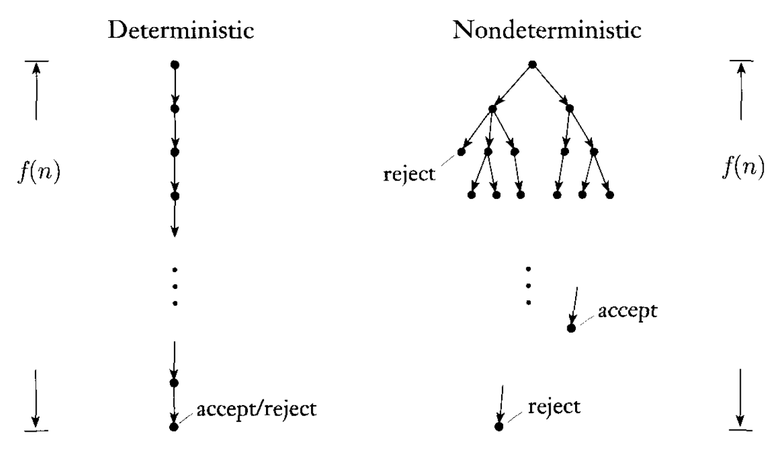
\includegraphics[width=0.5\linewidth]{Mdt e NMdt.png}
    \caption{Differenza tra MdT deterministica e non}
    \label{fig:enter-label}
\end{figure}

\begin{definition}
    Se un linguaggio $L\in \Sigma^*$ è deciso da una N-MdT M che opera in tempo $f(n)$ allora $L\in NTIME(f(n))$. 
\end{definition}

\section{Classe di complessità P ~\cite{5}} 
\begin{definition}
    La classe di complessità P è l'insieme di tutti i linguaggi che possono essere decisi in tempo polinomiale, ovvero:
    $$
    P = \bigcup_k \ TIME(n^k)
    $$
\end{definition}

\section{Classe di complessità NP \cite{5}}
\begin{definition}
    La classe di complessità NP è l'insieme di tutti i linguaggi che possono essere decisi in tempo polinomiale da una macchina non deterministica, ovvero:
    $$
    NP = \bigcup_k \ NTIME(n^k)
    $$
\end{definition}

\section{Riduzioni polinomiali}
La tecnica per dimostrare che un problema $P_2$ non può essere risolto in tempo polinomiale è la riduzione di un problema $P_1$, che si sa non essere $\mathcal{P}$, a $P_2$. 
Bisogna, però, richiedere un ulteriore vincolo: la traduzione da $P_1$ a $P_2$ deve richiedere un tempo polinomiale nella lunghezza dell'input.
 
\section{Problemi NP-completi e NP-hard}
\begin{definition}
    Diciamo che $L$ è $NP-$completo se:
    \begin{itemize}
        \item $L$ è in $NP$;
        \item per ogni linguaggio $L'$ in $NP$ esiste una riduzione polinomiale di $L'$ a $L$;
    \end{itemize}
\end{definition}

Su alcuni problemi $L$, sebbene sia possibile dimostrare la seconda condizione non è possibile dimostrare la prima, ovvero che $L\in NP$, tali problemi prendono il nome di NP-hard. 

\section{Il problema SAT}
Il problema di soddisfacibilità booleana, detto più comunemente SAT, è un esempio di problema NP-completo. 
\hfill \break
Il problema si basa sull'andare a decidere se un'espressione booleana è soddisfacibile. 

\hfill \break 
Le espressioni booleane sono formate da: 
\begin{itemize}
    \item variabili a valori booleani ovvero 1 per indicare true e 0 per indicare false; 
    \item gli operatori binari $\land$ e $\lor$ per indicare rispettivamente AND e OR;
    \item l'operatore unario $\lnot$ che indica la negazione logica; 
    \item parentesi per raggruppare il tutto; 
\end{itemize}

\begin{example}
    Un esempio di espressione booleana è $x \land \lnot(y \lor z)$.
\end{example}

\begin{definition}
    Un assegnamento di valori di verità per un espressione booleana E assegna i valori vero o falso a ognuna delle variabili presenti in E, di conseguenza il valore dell'espressione E a seguito dell'assegnamento T è indicato con $E(T)$.
    Se $E(T)=1$ allora l'espressione è soddisfatta, senò no.
\end{definition}

\noindent Il problema della soddisfacibilità è definito come:
 \begin{itemize}
     \item un'espressione booleana assegnata è soddisfacibile?
 \end{itemize}

Enunciato come linguaggio, SAT è l'insieme delle espressioni booleane soddisfacibili. 

Bisogna però trovare un modo per codificare il SAT. 
In un espressione booleana possono esserci un numero infinito di simboli, bisogna ideare un codice con un alfabeto finito per rappresentare espressioni che possono essere infinitamente grandi. 
Per farlo: 
\begin{itemize}
    \item rappresentiamo gli operatori binari e unari da se stessi ($\lnot, \land,\lor$);
    \item rappresentiamo la variabile $x_i$ come $x$ seguito dalla codifica binaria di $i$;
\end{itemize}

\begin{example}
    Ad esempio $\lnot x_1\land (x_2\lor x_3)$ equivale a $\lnot x1 \land(x10\lor x11)$ 
\end{example}

\subsection{NP-completezza del problema SAT}
Per dimostrare la NP-completezza di SAT andiamo a usare la riduzione per ridurre un qualsiasi linguaggio NP (accettato da un N-MdT in tempo polinomiale) a SAT. Per provare che SAT è NP-completo bisogna provare che: 

\begin{enumerate}
    \item SAT sta in NP;
    \item qualsiasi altro linguaggio in NP è riducibile a SAT; 
\end{enumerate}

\begin{proof}
Dimostriamo che SAT è NP-completo: 
    \begin{enumerate}
        \item Per provare che SAT è NP sfruttiamo una N-MdT. Supponiamo di avere un espressione booleana E e una macchina di Turing non deterministica M. Costruiamo M in modo tale che grazie al non determinismo provi tutti gli assegnamenti possibili di valori di verità in E. Ogni diramazione rappresenta quindi il tentativo di un diverso assegnamento di valori. Si possono raggiungere $2^n$ ID, ovvero configurazioni diverse e a questo punto basta valutare E per l'assegnamento di valori fatto (in ogni diramazione), se $E(T)=1$ allora accettiamo. Una N-MdT multinastro effettua la valutazione in tempo $O(n^2)$ mentre una singolo nastro in tempo $O(n^4)$, che è comunque polinomiale. 
        \item Sia $L$ un linguaggio qualsiasi appartenente a NP. Per definizione, esiste una macchina di Turing non deterministica $M$ che decide $L$ in tempo polinomiale $p(n)$. L'idea della riduzione è costruire, a partire da un'istanza $x$ di $L$, una formula booleana $\varphi_x$ tale che:\[\varphi_x \text{ è soddisfacibile } \iff x \in L.\] La costruzione avviene codificando il calcolo di $M$ su input $x$ in una tabella \textit{tempo × spazio}, dove ogni cella rappresenta il contenuto di un nastro, lo stato della macchina e la posizione della testina in un determinato passo. Le condizioni di correttezza del calcolo (transizioni valide, stato iniziale corretto, stato finale accettante) vengono espresse tramite vincoli booleani. La formula risultante $\varphi_x$ ha dimensione polinomiale rispetto a $|x|$ e può essere costruita in tempo polinomiale. Pertanto, ogni problema in NP si riduce in tempo polinomiale a SAT. ~\cite{7}
    \end{enumerate}
\end{proof}

\subsection{Variante di SAT: 3SAT}
Una versione ristretta del problema SAT molto utilizzata in Informatica è la variante 3SAT. 
Anche questo è un problema di soddisfacibilità booleana ma dove le espressioni booleane sono congiunzioni di disgiunzioni di esattamente tre variabili. 
Formalmente il 3SAT prende in input istanze di SAT in cui ogni clausola consta di esattamente 3 elementi e si pone come problema quello di stabilire, come per SAT, se esiste un assegnamento che rende vera la formula. 


\begin{example}
    Un esempio di espressione $E$ che rispetta le ipotesi di 3SAT è $(x_1 \lor x_2 \lor \lnot x_3) \land (\lnot x_1 \lor x_2 \lor x_3$). 
\end{example}

\begin{theorem}
    3SAT, come SAT, è NP-completo. 
\end{theorem}
\begin{proof}
    L'appartenenza a NP si mostra in quanto ogni istanza di 3SAT è anche istanza di SAT.
    Abbiamo già dimostrato che ogni problema in NP si può ridurre a SAT, mostriamo che ogni problema NP si può ridurre a 3SAT mostrando che SAT si può ridurre a 3SAT (SAT $\preceq$ 3SAT).
    Per farlo ci basta tradurre ogni clausola $l_1\lor...\lor l_m$ in una clausola uguale di 3SAT:
    \begin{itemize}
        \item se m=1: la trasformo in $l_1 \lor l_1 \lor l_1$;
        \item se m=2: la trasformo in $l_1 \lor l_2 \lor l_2$;
        \item se m=3: la tengo così com'è; 
        \item se m$>$3: introduco una nuova variabile X e restituisco $l_1 \lor l_2 \lor X$ e $\lnot X \lor l_4 \lor ... \lor l_m$ e riapplico la regola;
    \end{itemize}
\end{proof}

\section{3-Dimensional Matching (3DM) ~\cite{6}} 
Dati 3 insiemi disgiunti X,Y,Z di uguale dimensione $n$.
Dato un insieme di triple $T\subseteq X \times Y \times Z$.
Esiste un sottoinsieme $S\subseteq T$ tale che ogni elemento $\in X \cup Y \cup Z$ è in esattamente una tripla $s \in S$. 

\begin{theorem}
    3DM è NP-completo.
\end{theorem}
\begin{proof}
    Per dimostrare la NP-completezza di 3DM dobbiamo dimostrare sia che 3DM appartiene a NP, sia che ogni problema in NP è riducibile a 3DM. 
    La seconda parte la dimostriamo dimostrando che 3SAT è riducibile a 3DM e siccome abbiamo già dimostrato che SAT è riducibile a 3SAT e SAT soddisfa l'ipotesi, allora anche 3DM la soddisfa. 
    \begin{itemize}
        \item per dimostrare che 3DM appartiene a NP basta considerare un algoritmo non deterministico che crea un sottoinsieme di triple e in tempo polinomiale verifica che nessuna delle triple sia intersecata;
        \item riduciamo 3SAT a 3DM. Sia $U=\{u_1,u_2,...,u_n\}$ l'insieme delle variabili e sia $C=\{c_1,c_2,...,c_m\}$ l'insieme delle clausole.
        Cerchiamo di costruire 3 insiemi disgiunti $X,Y,Z$ e un insieme $M \subseteq X \times Y \times Z$ tale che M contenga una tripla se e solo se tutte le clausole di $C$ sono soddisfacibili.
        L'insieme delle triple M può essere visto come partizionato in 3 parti che possiamo definire variable gadget, clause gadget e garbage collection. La prima componente corrisponde alle singole variabili $u\in U$, per ognuna di esse vengono creati due elementi $y_{u_i}\in Y$ e $z_{u_i} \in Z$ che vanno a creare una tripla insieme a $u_i$. In questo caso si veranno a creare $2nu_i$ triple dove $nu_i$ rappresenta il numero di clausole in cui è presente la variabile $u_i$. Il tutto può essere rappresentato attraverso un grafo sul quale veranno mappate le variabili $u_i$ e le loro negazioni $\lnot u_i$, si ottiene una situazione rappresentabile come: 
        \begin{figure}[H]
            \centering
            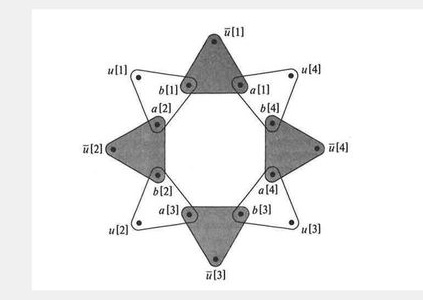
\includegraphics[width=0.5\linewidth]{variablegadget.jpeg}
            \caption{Truth setting component o variable gadget}
            \label{fig:enter-label}
        \end{figure}
        Si ottengono in questo modo due insiemi: 
        $$
        %\begin{align}
        T_i^t = \{(\lnot u_i, y_{u_i}, z_{u_i})\} \\
        T_i^f = \{(u_i, y_{u_i}, z_{u_{i+1}})\} \\
        %\end{align}
        $$
        $$
        T = T_i^f \cup T_i^t
        $$
        Si nota quindi che in ogni caso, per non sovrapporre gli elementi, si dovranno scegliere o i triangoli che contengono il valore positivo $u_i$ o la sua negazione, questo obbliga a scegliere un valore di verità per una delle variabili. 
        Allo stesso modo si crea la variable gadget, dove ogni variabile forma una tripla con due nuove variabili $y_c, z_c$ per ogni clausola $c_j \in C$ presente in $E$, questo per indicare quali variabili appaiono in quali clausole, si forma quindi: 
        $$
        C_j = \{(u_{ij},y_{c_j}, z_{c_j}): u_i \in c_j\} \cup \{(\lnot u_{ij},y_{c_j}, z_{c_j}): u_i \in c_j\}
        $$
        Per completare la costruzione viene usata la garbage collection che unisce ogni variabile ($u_i$) e la sua negazione ($\lnot u_i$) a due componenti $y_{g_k}\in Y$ e $z_{g_k}\in Z$, in questo modo tutti gli elementi che non appaiono in variable gadget o in clause gadget possono essere recuperate sfruttando la garbage collection: 
        $$
        G = \{(u_{ij},y_{g_k}, z_{g_k}), (\lnot u_{ij}, y_{g_k}, z_{g_k})\}
        $$
        Infine, creando un insieme di triple in modo che ogni elemento di $X \times Y \times Z$ appaia esattamente in una sola tripla:
        $$
        M = (\bigcup_{i=1}^{n}T_i) \cup (\bigcup_{j=1}^mC_j) \cup G
        $$
        abbiamo ridotto il problema di SAT a 3DM. 
    \end{itemize}
\end{proof}

\section{3-Exact-Cover (X3C)}
Sia $X$ un insieme finito con $|X|=3q$ elementi e una collezione $C$ di sottoinsiemi di 3 elementi di $X$ ci chiediamo se $C$ contiene una exact cover per X, cioè, se esiste una collezione $C' \subseteq C$ tale che ogni elemento di $X$ appare esattamente una volta in $C'$.

Si noti che 3DM non è altro che una versione ristretta di X3C.

Infatti è possibile ridurre il problema del 3DM a 3XC.

Sia $C = \{\{x,y,z\}: (x,y,z) \in T\}$ e sia $k = |X| =|Y|=|Z|=n$. 
Otteniamo che $C$ è una collezione di sottoinsiemi di $T$ dove $T$ è l'insieme delle triple di valori e $k$ rappresenta il numero di sottoinsiemi di $C$, ovvero $|C'|=k$, cioè ogni tripla rappresenta un sottoinsieme di $C$, ciò che vogliamo è che ogni elemento di $C'$ sia una tripla disgiunta. 
Supponiamo $M$ sia la soluzione al 3DM. 
Sia $C' = \{\{x,y,z\}: (x,y,z)\in M\}$, abbiamo $|M|=n=|C'|$. 
Sappiamo che se $(x,y,z)$ e $(x',y',z')$ sono due elementi distinti di $M$ allora, siccome per definizione $X\cap Y \cap Z = \emptyset$ avremmo $\{x,y,z\} \cap \{x',y',z\} = \emptyset$. 
Cioè gli elementi in $C'$ sono a due a due disgiunti, e siccome coprono tutti gli elementi dell'insieme universo, otteniamo che $C'$ è una soluzione al 3XC. 

Allo stesso modo, supponiamo $C'=\{C_1,C_2,...,C_k\}$ sia una soluzione al 3XC.
Sia $M=\{(x,y,z): \{x,y,z\} = C_i \ per \ i = 1,2,...k \}$.
Siccome gli $C_i'$ sono a due a due disgiunti, se $(x,y,z)$ e $(x',y',z')$ sono due elementi distinti di $M$ allora sono tutti distinti. 
Quindi $M$ è una soluzione al 3DM. 

Avendo quindi dimostrato che 3DM è un problema NP-completo, si dimostra che anche X3C lo è. 

